\documentclass{beamer}

\usepackage[utf8]{inputenc}
\usepackage[T1]{fontenc}
\usepackage{lmodern,tgadventor}
\usepackage{textcomp}
\usepackage{tikz}
\usetikzlibrary{backgrounds,decorations.text,fadings,trees}

\useinnertheme{rectangles}
\usecolortheme[accent=red]{solarized}
\beamertemplatenavigationsymbolsempty
\setbeamertemplate{footline}[frame number]

\newcommand\commit[2]{\node[commit] (#1) {};%
                      \node[clabel] (#1 label) at (#1) {\texttt{#1}: #2};}
\newcommand\ghost[1]{\coordinate (#1);}
\newcommand\connect[2]{\path[connections] (#1) to[out=90,in=-90] (#2);}
\newcommand\gittag[1]{%
 \begin{tikzpicture}[baseline]
  \node[fill=solarizedRebase02, rounded corners, inner sep=1pt, anchor=base] {
    \color{solarizedYellow}\vphantom{|}#1
   };
 \end{tikzpicture}%
}
\newcommand\branch[1]{%
 \begin{tikzpicture}[baseline]
  \node[fill=solarizedRebase02, rounded corners, inner sep=1pt, anchor=base] {
    \color{solarizedRed}\vphantom{|}#1
   };
 \end{tikzpicture}%
}

% http://tex.stackexchange.com/questions/55806/tikzpicture-in-beamer/55827#55827
\tikzset{
  invisible/.style={opacity=0},
  visible on/.style={alt=#1{}{invisible}},
  alt/.code args={<#1>#2#3}{%
    \alt<#1>{\pgfkeysalso{#2}}{\pgfkeysalso{#3}}
  },
}

\author{Elliott Sales de Andrade}
\title{CIG Seismo Code on Git/GitHub}
\institute{University of Toronto}
\titlegraphic{%
 \begin{tikzpicture}[
    commit/.style={draw, circle, fill=solarizedViolet, inner sep=0pt,
                   minimum size=5pt},
    clabel/.style={right, outer sep=1em},
    connections/.style={draw, solarizedViolet}
  ]
  \useasboundingbox (-1,1em) rectangle (1,8em); % Mysteriously chosen to fit...
  \matrix [column sep={1em,between origins}, row sep=\lineskip,
           ampersand replacement=\&]%
  {
   \commit{cd83b68}{\gittag{v6.0.0} \branch{master} submodules updated} \& \& \\
   \commit{170e5f7}{Update submodules in master} \& \& \\
   \commit{c0bc5ba}{Merge remote-tracking branch `origin/devel'} \& \& \\
   \& \commit{754300e}{Update README.md} \& \\
   \& \commit{40bcfdd}{Merge pull request \#68 from QuLogic/readme} \& \\
   \& \& \commit{e2f2928}{section-ify readme file.} \\
   \& \& \commit{eb6066e}{change to markdown so github linkifies stuff.} \\
   \& \& \commit{5babcb0}{add links to submodules in readme.} \\
   \& \commit{2b70a18}{merge pull request \#67 from komatits/devel} \& \\
   \ghost{5e338b5} \& \& \\
  };
  \connect{170e5f7}{cd83b68};
  \connect{c0bc5ba}{170e5f7};
  \connect{754300e}{c0bc5ba};
  \connect{40bcfdd}{754300e};
  \connect{e2f2928}{40bcfdd};
  \connect{eb6066e}{e2f2928};
  \connect{5babcb0}{eb6066e};
  \connect{2b70a18}{5babcb0};
  \connect{2b70a18}{40bcfdd};
  \connect{5e338b5}{2b70a18};
  \connect{5e338b5}{c0bc5ba};
  \fill [color=solarizedRebase03, path fading=north] (-6,-1.1) rectangle (6,.8);
 \end{tikzpicture}%
}

\begin{document}

\begin{frame}[plain,noframenumbering]
 \titlepage
\end{frame}

\begin{frame}
 \frametitle{Outline}
 \tableofcontents
\end{frame}

\section{Introduction}

\begin{frame}
 \frametitle{Introduction}

 \begin{itemize}
  \item CIG is transitioning code from Subversion to Git
  \item Also shifting most hosting to \href{https://github.com/}{GitHub}
  \item All Seismology code has been migrated:
   \begin{itemize}
    \item \href{https://github.com/geodynamics/specfem1d}{Specfem1D}
    \item \href{https://github.com/geodynamics/specfem2d}{Specfem2D}
    \item \href{https://github.com/geodynamics/specfem3d}{Specfem3D}
    \item \href{https://github.com/geodynamics/specfem3d_globe}{Specfem3D Globe}
    \item \href{https://github.com/geodynamics/mineos}{Mineos}
    \item \href{https://github.com/geodynamics/flexwin}{Flexwin}
    \item \href{https://github.com/geodynamics/axisem}{AxiSEM}
   \end{itemize}
  \item Also code for
        \href{http://geodynamics.org/cig/software/\#cs}{Computational Science},
        \href{http://geodynamics.org/cig/software/\#geodyn}{Geodynamo},
        \href{http://geodynamics.org/cig/software/\#long}{Long-Term Tectonics},
        \href{http://geodynamics.org/cig/software/\#mc}{Mantle Convection},
        \href{http://geodynamics.org/cig/software/\#short}{Short-Term Crustal
        Dynamics}
 \end{itemize}
\end{frame}

\subsection{What is Git?}

\begin{frame}
 \frametitle{Introduction}
 \framesubtitle{What is Git?}

 The stupid content tracker\footnotemark
 \begin{itemize}
  \item \href{http://git-scm.com/about/distributed}{Distributed}
   \begin{itemize}
    \item Multiple backups
    \item Flexible workflow
   \end{itemize}
  \item \href{http://git-scm.com/about/branching-and-merging}{Quick and easy
        branching}
   \begin{itemize}
    \item Frictionless context switching
    \item Role-based codelines
    \item Feature based workflow
    \item Disposable experimentation
   \end{itemize}
  \item \href{http://git-scm.com/about/small-and-fast}{Small and fast}
        --- One or two orders of magnitude faster than SVN (except cloning)
  \item \href{http://git-scm.com/about/info-assurance}{Repository integrity}
        --- Files, commit messages, dates
  \item \href{http://git-scm.com/about/staging-area}{Staging area}
        --- Flexible committing
  \item \href{http://git-scm.com/about/free-and-open-source}{Free and open
        source} --- GNU GPL 2.0
 \end{itemize}

 \footnotetext{\url{http://git-scm.com/about/}}
\end{frame}

\subsection{What is GitHub?}

\begin{frame}
 \frametitle{Introduction}
 \framesubtitle{What is GitHub?}

 Provides hosting and resources for open source software:
 \begin{itemize}
  \item Issue tracking
   \begin{itemize}
    \item Tasks
    \item Features
    \item Pull requests
    \item etc.
   \end{itemize}
  \item Code review
   \begin{itemize}
    \item Commit comments,
    \item Pull requests,
    \item Diffs,
    \item etc.
   \end{itemize}
  \item Wikis
  \item Collaborative tools
  \item Statistics
 \end{itemize}
\end{frame}

\subsection{Version Control Basics}

%
% SVN Checkout
%

\begin{frame}
 \frametitle{Version Control with Subversion}
 \framesubtitle{Checkout}

 \begin{columns}
  \begin{column}{0.3\textwidth}
   \begin{tikzpicture}[
      remember picture,
      show background rectangle,
      commit/.style={draw, rectangle, rounded corners, fill=solarizedRebase02,
                     inner sep=1pt, minimum width=1.5em},
      connections/.style={draw}
    ]
    \matrix [column sep={1em,between origins}, row sep={1.5em,between origins},
             ampersand replacement=\&]%
    {
     \ghost{name}; \\
     \node[commit, visible on=<3->] (9) {9}; \\
     \node[commit, visible on=<3->] (8) {8}; \\
     \node[commit] (7) {7}; \\
     \node[commit] (6) {6}; \\
     \node[commit] (5) {5}; \\
     \node[commit] (4) {4}; \\
     \node[commit] (3) {3}; \\
     \node[commit] (2) {2}; \\
     \ghost{1}; \\
    };
    \node[anchor=south,align=center] at (name) {Central\\Repository};
    \foreach \x in {3,...,7} {
     \pgfmathparse{int(\x-1)}
     \connect{\pgfmathresult}{\x};
    }
    \path[connections, densely dashed] (1) -- (2);
    \path[connections, visible on=<3->] (7) -- (8);
    \path[connections, visible on=<3->] (8) -- (9);
   \end{tikzpicture}
  \end{column}
  \begin{column}{0.5\textwidth}
   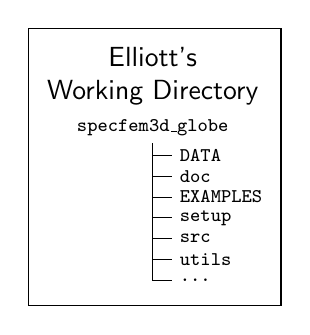
\begin{tikzpicture}[%
      remember picture,
      show background rectangle,
      background rectangle/.style={draw, visible on=<4->},
      visible on=<4->,
      every node/.style={anchor=west, minimum height=1em,
                         font={\scriptsize\ttfamily}, inner sep=2.5pt},
      every edge/.style={thick},
      root/.style={},
      grow via three points={one child at (0.25,-1em) and
                             two children at (0.25,-1em) and (0.25,-1.75em)},
      edge from parent path={(\tikzparentnode.south) |- (\tikzchildnode.west)}
    ]
    \node [root] (E root) {specfem3d\_globe}
     child { node {DATA} }
     child { node {doc} }
     child { node {EXAMPLES} }
     child { node {setup} }
     child { node {src} }
     child { node {utils} }
     child { node {\dots} };
    \node[anchor=south, font={\sffamily}, align=center] at (E root.north)
     {Elliott's\\Working Directory};
   \end{tikzpicture}

   \hfill
   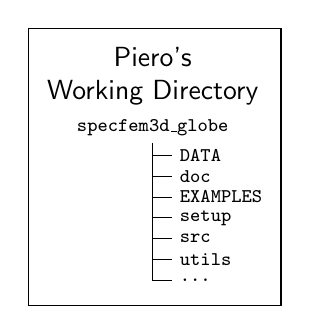
\begin{tikzpicture}[%
      remember picture,
      show background rectangle,
      background rectangle/.style={draw, visible on=<2->},
      visible on=<2->,
      every node/.style={anchor=west, minimum height=1em,
                         font={\scriptsize\ttfamily}, inner sep=2.5pt},
      every edge/.style={thick},
      root/.style={},
      grow via three points={one child at (0.25,-1em) and
                             two children at (0.25,-1em) and (0.25,-1.75em)},
      edge from parent path={(\tikzparentnode.south) |- (\tikzchildnode.west)}
    ]
    \node [root] (P root) {specfem3d\_globe}
     child { node {DATA} }
     child { node {doc} }
     child { node {EXAMPLES} }
     child { node {setup} }
     child { node {src} }
     child { node {utils} }
     child { node {\dots} };
    \node[anchor=south, font={\sffamily}, align=center] at (P root.north)
     {Piero's\\Working Directory};
   \end{tikzpicture}
  \end{column}
 \end{columns}

 \begin{tikzpicture}[
    remember picture, overlay,
    path/.style={thick, ->},
    label/.style={decorate, decoration={text along path, text align=center,
                                        text color=solarizedRebase0,
                                        transform={yshift=1pt},
                                        text={svn checkout}}}
  ]
  \draw<2->[path] (7.east) to[out=0,in=180] (P root.west);
  \draw<2>[label] (7.east) to[out=0,in=180] (P root.west);
  \draw<4->[path] (9.east) to[out=0,in=180] (E root.west);
  \draw<4->[label] (9.east) to[out=0,in=180] (E root.west);
 \end{tikzpicture}
\end{frame}

%
% SVN Commit
%

\begin{frame}
 \frametitle{Version Control with Subversion}
 \framesubtitle{Commits}

 \begin{columns}
  \begin{column}{0.3\textwidth}
   \begin{tikzpicture}[
      remember picture,
      show background rectangle,
      commit/.style={draw, rectangle, rounded corners, fill=solarizedRebase02,
                     inner sep=1pt, minimum width=1.5em},
      connections/.style={draw}
    ]
    \matrix [column sep={1em,between origins}, row sep={1.5em,between origins},
             ampersand replacement=\&]%
    {
     \node[commit, visible on=<3->] (repository) {10}; \\
     \node[commit] (9) {9}; \\
     \node[commit] (8) {8}; \\
     \node[commit] (7) {7}; \\
     \node[commit] (6) {6}; \\
     \node[commit] (5) {5}; \\
     \node[commit] (4) {4}; \\
     \node[commit] (3) {3}; \\
     \node[commit] (2) {2}; \\
     \ghost{1}; \\
    };
    \node[anchor=south, align=center] at (repository) {Central\\Repository};
    \foreach \x in {3,...,9} {
     \pgfmathparse{int(\x-1)}
     \connect{\pgfmathresult}{\x};
    }
    \path[connections, densely dashed] (1) -- (2);
    \path[connections, visible on=<3->] (9) -- (repository);
   \end{tikzpicture}
  \end{column}
  \begin{column}{0.5\textwidth}
   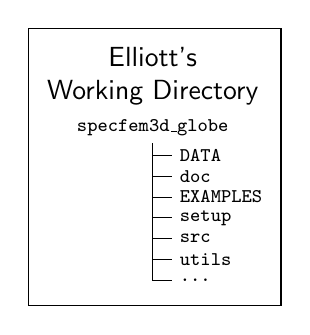
\begin{tikzpicture}[%
      remember picture,
      show background rectangle,
      every node/.style={anchor=west, minimum height=1em,
                         font={\scriptsize\ttfamily}, inner sep=2.5pt},
      every edge/.style={thick},
      root/.style={},
      grow via three points={one child at (0.25,-1em) and
                             two children at (0.25,-1em) and (0.25,-1.75em)},
      edge from parent path={(\tikzparentnode.south) |- (\tikzchildnode.west)}
    ]
    \node [root] (E root) {specfem3d\_globe}
     child { node {DATA} }
     child { node {doc} }
     child { node {EXAMPLES} }
     child { node {setup} }
     child { node {src} }
     child { node {utils} }
     child { node {\dots} };
    \node[anchor=south, font={\sffamily}, align=center] at (E root.north)
     {Elliott's\\Working Directory};
   \end{tikzpicture}

   \hfill
   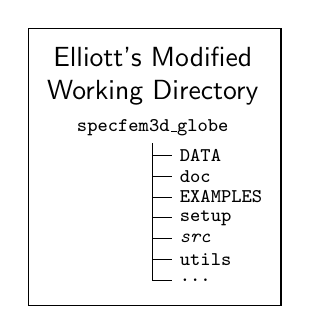
\begin{tikzpicture}[%
      remember picture,
      show background rectangle,
      background rectangle/.style={draw,visible on=<2-3>},
      visible on=<2-3>,
      every node/.style={anchor=west, minimum height=1em,
                         font={\scriptsize\ttfamily}, inner sep=2.5pt},
      every edge/.style={thick},
      root/.style={},
      grow via three points={one child at (0.25,-1em) and
                             two children at (0.25,-1em) and (0.25,-1.75em)},
      edge from parent path={(\tikzparentnode.south) |- (\tikzchildnode.west)}
    ]
    \node [root] (M root) {specfem3d\_globe}
     child { node {DATA} }
     child { node {doc} }
     child { node {EXAMPLES} }
     child { node {setup} }
     child { node {\itshape src} }
     child { node {utils} }
     child { node {\dots} };
    \node[anchor=south, font={\sffamily}, align=center] at (M root.north)
     {Elliott's Modified\\Working Directory};
   \end{tikzpicture}
  \end{column}
 \end{columns}

 \begin{tikzpicture}[
    remember picture, overlay,
    path/.style={thick, ->},
    label/.style={decorate, decoration={text along path, text align=center,
                                        text color=solarizedRebase0}}
  ]
  \draw<1-3>[path] (9.east) to[out=0,in=180] (E root.west);
  \draw<2-3>[path] (E root.east) to[out=0,in=0] (M root.east);
  \draw<2>[label, decoration={transform={yshift=1pt}, text={Editing}}]
   (E root.east) to[out=0,in=0] (M root.east);
  \draw<3>[path] (M root.west) to[out=180,in=0] (repository.east);
  \draw<3>[label, decoration={transform={yshift=-1em}, text={svn commit}}]
   (repository.east) to[out=0,in=180] (M root.west);
  \draw<4->[path] (repository.east) to[out=0,in=180] (E root.west);
 \end{tikzpicture}
\end{frame}

\section{Using CIG Code from Git}

\section{Local Development}

\section{Contributing Code}

\section{Additional Information}

\begin{frame}
 \frametitle{Additional Information}

 \begin{itemize}
  \item \href{http://www.vogella.com/tutorials/Git/article.html}{\textit{Git - Tutorial}}
   by Lars Vogel
  \item \href{http://www.git-tower.com/blog/git-cheat-sheet/}{\textit{Git Cheat Sheet}}
  \item \href{https://github.com/geodynamics/specfem3d/wiki/Git-tips-for-developers}{\textit{Git tips for developers}}
   on Specfem3D wiki
  \item \href{http://git-scm.com/book}{\textit{Pro Git book}}
  \item \href{https://try.github.io/levels/1/challenges/1}{\textit{Try Git}}
   in your browser
 \end{itemize}
\end{frame}

\end{document}
